%8
\documentclass[output=paper]{LSP/langsci}
\author{Justin T. McBride}
\title{Reconstructing post-verbal negation in {Kansa}: {A} pedagogical problem}
\abstract{Despite the fact that there are no L1 speakers of \il{Kanza}Kansa, and the handful of learners are mostly novice-range speakers, the Kaw Nation has been actively engaged in \is{language revitalization}revitalization efforts for many years. The absence of speaker knowledge poses a major problem for \is{curriculum development}curriculum developers insofar as the quality of Kansa \isi{pedagogical materials} is often limited to what can be uncovered from analysis of documentary materials -- mostly those of Dorsey\ia{Dorsey, James Owen} and Rankin\ia{Rankin, Robert L.}. These sources, though essential, are far from complete. For instance, they lack many constructions that potential language learners would want to know, including how to express what in English is captured by the word \textit{wouldn't}. In such cases, \is{syntax}syntactic analysis can be used to reconstruct certain areas of Kansa grammar. Kansa is a left-branching, head-marking language with canonical (S)OV \isi{word order}. Several features of its syntax seem to complicate an X-Bar treatment of Kansa, but the placement of \isi{negation} (\textsc{neg}) in the post-verbal complex seems to violate a number of principles all at once. This gives rise to contradictory expectations for its location in different contexts. In this paper, I discuss one way of reconstructing Kansa \textsc{neg} to fill a pedagogical need. While not arriving at any definite theoretical conclusion, I do arrive at a possible one, and conclude with a set of recommendations for \is{curriculum development}curriculum developers dealing with this and other such problems. 
% KEYWORDS: [Kansa, negation, modality, language revitalization, reconstruction, syntax in language pedagogy]
} 
\ChapterDOI{10.17169/langsci.b94.171}

\maketitle

\begin{document}

\section{Introduction}
Among the many problems plaguing the \is{language revitalization}revitalization efforts of languages without L1 speakers is that a large number of the useful, conversational things that learners might want to say are simply unknown. These may include greetings and pleasantries, common expressions for introducing self and others, stating likes and dislikes, making and fulfilling requests for additional information, telling time, and so on -- all of which people use with great frequency in their own L1s and expect to be able to say in an L2. In fact, language teachers usually want to teach these sorts of conversational forms early on in classes as stock constructions that can build both competence and confidence in their learners. However, with no speakers around to ask, there may only be the products of linguistic research available as the next best thing. Perhaps there is a \isi{dictionary}, a text series\is{corpus}, or simply a set of field notes. Yet, even the most diligent field worker\is{field work} may not think to elicit very practical expressions such as `hello, my name is [blank],' `I did not understand what you said; please repeat it,' or `how do you say [blank] in the [blank] language?' 

The case of the \ili{Dhegiha} Siouan language Kansa (also known as \ili{Kanza} or Kaw) is precisely as described above. Dorsey's\ia{Dorsey, James Owen} 1880s-era \isi{field work} yielded a rather large set of slip files, two dozen texts collected from nine separate consultants, and hundreds of pages of ethnographic notes\is{corpus}, all of which Rankin\ia{Rankin, Robert L.} used in his own extensive work with the last \il{Kanza}Kansa speakers in the 1970s and early 1980s. Following the deaths of his consultants, Rankin continued working on \il{Kanza}Kansa for the rest of his life. Neither Dorsey\ia{Dorsey, James Owen} nor Rankin\ia{Rankin, Robert L.} intended their work to be used as-is for \is{language revitalization}revitalization and \isi{curriculum development} purposes, but this is what happened: Such efforts must begin somewhere, and their material was the logical starting point. Fortunately, Rankin was willing to contribute to this enterprise, and he often worked on Siouan language \is{pedagogical materials}pedagogy side-by-side with other linguists (these included myself and several other contributors to this volume), both in the classroom and behind the scenes. Yet, even with Rankin --- himself a lifelong educator --- and a team of Siouanists at the head of \il{Kanza}Kansa \isi{language classes}, the learner outcomes were often far less than could be expected of other beginning \isi{language classes}; the source material was simply incomplete. As a consequence, many basic things remain unknown for \il{Kanza}Kansa and, accordingly, unused among language learners.
 
Consider a common \ili{English} expression such as `She \textit{wouldn't} go, `Mike \textit{wouldn't} do that,' `they \textit{wouldn't} give it to me,' or the like. To my knowledge, there is no recorded translation of this expression in the available \il{Kanza}Kansa materials. I honestly cannot recall the exact circumstances of how this lacuna was discovered, but I remember that it came up in the Kaw Nation's Thursday night community language class\is{language classes} in Kaw City, Oklahoma, in the mid-2000s. Perhaps some thoughtful student simply asked, ``How do you say, `she wouldn't go,' in the language?'' Surely I knew that the answer to the question would involve post-verbal \isi{negation} and some use of both the potential and non-continuative enclitics, but I was flummoxed as to how to order these elements. Whatever the circumstances may have been, once it became apparent that I could not immediately provide an answer based on my working knowledge of \il{Kanza}Kansa \isi{syntax}, I probably explained that I would have to do more research and return with a definite solution later. Little did I know then that I \textit{wouldn't} have a satisfying answer the next week, month, or even year!

Part of the problem lies in just how one would go about trying to find the answer. It would ideally involve reviewing the available texts\is{corpus} and field elicitations with an eye toward finding how Dorsey\ia{Dorsey, James Owen}, Rankin\ia{Rankin, Robert L.}, or someone else may have recorded it. Those working on \il{Kanza}Kansa have, of course, done a great deal of secondary research like this; the lacunae are numerous, the learners are curious, and the available scholarly analysis is of high quality. Nevertheless, the construction does not appear in the materials. Failing that, the next step would involve reconstructing the form from a set of near-matches combined with knowledge of the language's \isi{syntax}. Yet, \isi{syntax} is one area where \il{Kanza}Kansa and the other \ili{Dhegiha} languages are not always described in the greatest detail. Both Rankin's brief grammatical sketch of \il{Kanza}Kansa \citeyear{Rankin1989} and his later sketch of \ili{Quapaw} \citeyear{Rankin2005b} discuss a variety of \isi{syntax} topics, as does \citegen{Quintero2004} book-length grammar of \ili{Osage}. But all of these works are overviews of \ili{Dhegiha} grammar, and are ultimately too general to offer fine-grained perspective on such a specific question. 

In this chapter, I will attempt a basic generative syntactic\is{syntax} analysis of \il{Kanza}Kansa post-verbal \isi{negation}. Bear in mind that I am ultimately looking for a pedagogical solution\is{pedagogical materials}, not a theoretical one. As such, I do not advocate any particular theory of formal \isi{syntax} and feel fairly free to borrow liberally from several eras of transformational grammar all at once. I am fully aware that this juxtaposition of concepts may make my analysis problematic for strict syntacticians, and perhaps also for dedicated pedagogues who may find any such analysis tedious to begin with. I do this not to alienate potential readers or to break any new theoretical ground, but simply to predict an unattested enclitic order using the formal means within my disposal. I also hope that my analysis and the discussion that follows will help to shed some light on a few philosophical principles that I consider very important to anyone working in Siouan languages:

\begin{itemize}
\item Gaps in the available documentation of languages\is{language documentation} are not necessarily insurmountable challenges;
\item Grammar must occasionally be reconstructed in order for it to be taught;
\item Formal analysis is not, by mere virtue of its formality, better than other means of acquiring grammatical knowledge; yet
\item Formal analysis of some manner or another can serve practical pedagogical purposes\is{pedagogical materials}.
\end{itemize}

\subsection{X-Bar considerations}
\il{Kanza}Kansa, like other \ili{Mississippi Valley Siouan} languages, particularly those of the \ili{Dhegiha} branch, is head-marking with a canonical (S)OV \isi{word order} (see, for example, \citet[421]{Quintero2004} for the \ili{Dhegiha} language \ili{Osage}; \citet[488--490]{Rankin2005b} for \ili{Quapaw}, also \ili{Dhegiha}; and \citet[369]{Cumberland2005} for \ili{Assiniboine}, a \ili{Dakotan} language). Moreover, it appears to follow the same sort of left-branching syntactic pattern that \citet{Boyle2007} described for \ili{Hidatsa} (\ili{Missouri Valley Siouan}). Although this paper is concerned with the \isi{syntax} of the \il{Kanza}Kansa post-verbal complex, it is important to point out some grammatical features that complicate an X-Bar analysis of \il{Kanza}Kansa, including those as follows.

\begin{description}
\item[(a)]	Left-branching: Tree structures for \il{Kanza}Kansa and the movement of elements within them appear to run counter to the right-branching patterns typical of X-Bar theory.

\item[(b)]	Radical pro-drop status: For the most part, only nominal subjects and objects appear independently in the sentence, the former presumably in the [SPEC,\is{specifier} TP]; all else is handled by verbal inflection\is{conjugation}. 

\item[(c)]	Concept of word: Just how much of enumeration and derivation is left up to morphology versus \isi{syntax} is essentially still up for grabs; as a consequence, so, too, are the classifications of enclitics, auxiliaries, affixes. 

\item[(d)]	Abstract tense: The TP in \il{Kanza}Kansa is at best misnamed given the language's general absence of tense marking, and the projection below the topmost \il{Kanza}Kansa CP is probably little more than an agreement-checking level.
\end{description}

These features are crucial to any full description of \il{Kanza}Kansa \isi{syntax}, and they have very interesting implications for syntactic theories as a whole. Nonetheless, while I take these points as fundamental assumptions for the analysis that follows, they are actually not altogether relevant for me to discuss in greater length given the narrow focus of this chapter.

\begin{figure}
\caption{\il{Kanza}Kansa aspect} \label{kansaaspect}
\Tree [ .Aspect [ .Simple [ .Continuative ] [ .Non-continuative ] ] [ .Augmented [ .Potential ] [ .{Habitual, Durative} ] ] ]
\end{figure}

\subsection{Aspect}
Tense may be absent in \il{Kanza}Kansa, but verbal aspect is quite developed. \figref{kansaaspect} shows the general division of aspect in \il{Kanza}Kansa. The primary division is between what I have termed simple and augmented aspect. Simple aspect is obligatory in all \isi{clauses} while augmented is not. Simple aspect is further divided into continuative/imperfect (\textsc{cont}) and non-continuative/perfect (\textsc{ncont}) aspects, which are in complementary distribution. \textsc{cont} is marked on verbs through a complex series of post-verbal enclitics (\citet[485]{Rankin2005b} argues that these enclitics ``are actually conjugated as fully-fledged auxiliary verbs'' in the closely related \ili{Dhegiha} language \ili{Quapaw}; see also \citet{Rankin2004positionals}, for a much more detailed discussion) that also carry with them a sense of the \isi{subject}'s physical orientation in space. These include such categories as \textsc{cont-lie}, \textsc{cont-sit}, \textsc{cont-stand}, \textsc{cont-move}, etc. Moreover, these auxiliaries agree with the phi features of the verbal \isi{subject}s. Non-continuative aspect (\textsc{ncont}), on the other hand, is marked in two ways: A null form (-$\varnothing$) is used with \textsc{1sg, 1du}, and \textsc{2sg} \isi{subject}s; the verbal enclitic \textit{-(a)be}\footnote{I have written the initial vowel in parentheses to avoid a digression into what is occasionally known as \isi{ablaut} in Siouan. Suffice it to say, this initial vowel surfaces only when the final vowel of the element to which it attaches ends in \textit{-e}, presumably due to a V1+V2=V2 rule involving \il{Kanza}Kansa /e/ and /a/. For a more detailed treatment of this phenomenon throughout Siouan, see \citet{Rankin1995}.}\footnote{Both to save space and to preserve consistency with source material where appropriate, all \il{Kanza}Kansa words in this chapter are written only in the practical \isi{orthography}. This system is phonological in nature, but uses fewer special characters, allows digraphs and trigraphs, and makes use of \ili{English}-based capitalization and punctuation standards that potential language learners may regard as normal.} is used with \textsc{1pl, 2pl}, and \textsc{3cn} subjects. This suggests a person and number configuration as shown in \figref{ncont}. The augmented division includes potential (\textsc{pot})\footnote{Note that \textsc{pot} is occasionally regarded in the Siouan literature as an irrealis marker (see \citealt{Quintero2004,Quintero2009}).} on the one hand and several habitual (\textsc{hab}) and durative (\textsc{dur}) aspects on the other. The features \textsc{hab} and \textsc{dur} function syntactically in the same way as \textsc{pot}. I classify these as augmented due to the fact that they can be combined as needed with either simple aspect to generate \isi{compound} aspects such as \textsc{pot cont}, \textsc{pot ncont}, \textsc{hab ncont}, etc. The feature \textsc{pot} consists of the underlying enclitic \textit{ce}, which only surfaces as such when no other post-verbal elements -- aspect or mood -- follow it; this is very rare, but it does occur. It most often takes the shape of \textit{ta} through a sequence of regular phonological changes.\footnote{The so-called \isi{ablaut} considerations mentioned in footnote 1 are presumably responsible for two allomorphs of the \textsc{pot} enclitic surfacing in different post-verbal phonetic environments. These forms include \textit{ce} and \textit{ta}, the former of which further exhibits routine spirantization of the initial stop before a front vowel.} Though the \isi{phonology} of this variation is understood, the mechanism behind it is not, a fact that raises some interesting questions about its enclitic status. Note that \figref{ncont} is concerned with the post-verbal arrangement of person and number considerations, and there are pronominal prefixes that are shared between numbers for the same person, including, for instance, for \textsc{1du} and \textsc{1pl} and for \textsc{2sg} and \textsc{2pl}.

\begin{figure}
\caption{Person and number categories in \il{Kanza}Kansa with respect to \textsc{ncont} marking} \label{ncont}

\begin{center}
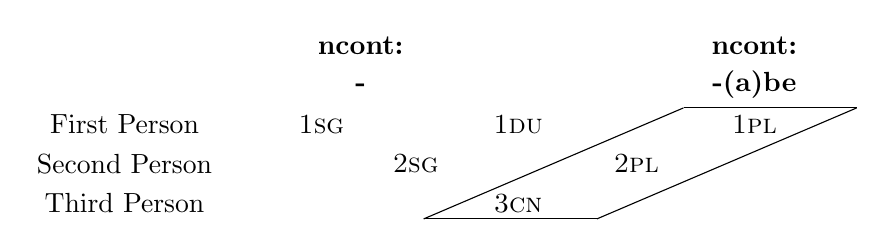
\begin{tikzpicture}

\draw (3,0) node {\textbf{\textsc{ncont}:}};
\draw (3,-0.5) node{\textbf{-$\varnothing$}};
\draw (8,0) node {\textbf{\textsc{ncont}:}};
\draw (8,-0.5) node {\textbf{-(a)be}};
\draw (0,-1) node {First Person};
\draw (2.5,-1) node {\textsc{1sg}};
\draw (5,-1) node {\textsc{1du}};
\draw (8,-1) node {\textsc{1pl}};
\draw (0,-1.5) node {Second Person};
\draw (3.7,-1.5) node {\textsc{2sg}};
\draw (6.5,-1.5) node {\textsc{2pl}};
\draw (0,-2) node {Third Person};
\draw (5,-2) node {\textsc{3cn}};

\draw (3.8,-2.2) -- (6,-2.2);
\draw (7.1,-0.79) -- (9.3,-0.79);
\draw (3.8,-2.2) -- (7.1,-0.79);
\draw (6,-2.2) -- (9.3,-0.79);

\end{tikzpicture}
\end{center}
\end{figure}

\subsubsection{\textsc{pot} enclitic status}

\textsc{pot}, unlike other post-verbal enclitics, is syntactically\is{syntax} dependent on what comes before it (it is enclitic to the main verb, presumably as the head of a PotP) but phonologically dependent on what comes after it (its shape is determined by its proximity to the end of the clause). Furthermore, owing perhaps to its consonantal rather than vocalic onset,\footnote{The other augmented aspect enclitics, \textsc{hab} and \textsc{dur}, also feature consonantal onsets, a fact that may strengthen the notion of augmented aspect as a natural class in \il{Kanza}Kansa.} it does not interact phonologically with the main verb. As such, the \textsc{pot} enclitic is somewhat different from that of, say, \textsc{ncont}.\footnote{The fact is represented in the \il{Kanza}Kansa practical \isi{orthography} by a space between the main verb and \textsc{pot} where no such space is left between the main verb and \textsc{ncont}.}

\subsubsection{Aspect order} 

The \isi{clauses} in example \REF{postverbalorder} and their templatic arrangement in \tabref{postverbalordertable} illustrate some representative combinations of the major aspects and the order in which they typically occur post-verbally.\footnote{In this paper, I mark pronouns using \textsc{agt} for agent and \textsc{pat} for patient, without regard to the various inflectional\is{conjugation} realizations found throughout \ili{Dhegiha}; the use of null pronouns in third person makes the classification as agent or patient irrelevant. I mark number using \textsc{sg} for singular, \textsc{du} for inclusive dual, and \textsc{pl} for plural. I also use \textsc{cn}, after Kelly's (\citeyear{Kelly1992}) \ili{Hebrew} \isi{gender} convention, to represent so-called common number in third person where singular and plural have collapsed in \il{Kanza}Kansa.} \footnote{All clausal\is{clauses} examples in this paper come from sentences in  \citet{McBrideCumberland2009}, \textit{Compiled \ili{Kanza} texts}, or \citet{McBrideCumberland2010}, \textit{\ili{Kanza} reader}, abbreviated CKT and KR, respectively. Corresponding page numbers appear after the \ili{English} glosses.} \footnote{The analysis of pronominals here differs from that presented either in \citet{Quintero2004} or \citet{Rankin2005b}, where all \textsc{1sg.agt} and \textsc{2sg.agt} pronominals are represented by archiphonemic WA- and YA-, respectively, and phonological rules are needed to explain their phonetic realization. To simplify things, I have simply shown final realizations in the analysis.}

\ea\label{postverbalorder}

\ea\label{postverbalorder1}{Wipághe tá miⁿkhe.\\ 
\gll
$\varnothing$-\textit{wi-p-(g)aghe}  \textit{ta}  \textit{miⁿkhe} \\
 \textsc{3cn-2cn.pat-1sg.agt-1sg.cont.sit}   \textsc{pot}   \textsc{1sg.agt}.make \\
\glt  `I will make them for you' (KR, p. 192) \\
}

\ex\label{postverbalorder2}{Yuz\'e ta akhá.\\ 
\gll
$\varnothing$-$\varnothing$-\textit{yuze}   \textit{ta}  \textit{akha} \\
\textsc{3cn-3cn}-take  \textsc{pot}  \textsc{3cn.cont.rest} \\
\glt  `S/he was about to take it.' (KR, p. 200) \\
}

\ex\label{postverbalorder3}{Hne tábe.\\ 
\gll
\textit{hn-(y)e} 	 \textit{ta}	 -\textit{(a)be} \\
\textsc{2pl.agt}-go  \textsc{pot}  \textsc{-ncont} \\
\glt  `You (\textsc{pl}) will have gone.' (KR, p. 192)\\
}

\ex\label{postverbalorder4}{Ozhú tábe.\\ 
\gll
\textit{o}-$\varnothing$-$\varnothing$-\textit{zhu} 	 \textit{ta}	 -\textit{(a)be} \\
in-\textsc{3cn-3cn}-pour 	\textsc{pot}  \textsc{-ncont} \\
\glt  `S/he would plant it.' (KR, p. 111) \\
}
\z
\z

\begin{table}
\caption{Order of post-verbal aspect elements} \label{postverbalordertable}
\begin{tabular}[h!]{ l l l l }
\lsptoprule
example & V& \textsc{pot} & \textsc{cont/ncont} \\
\midrule 
\REF{postverbalorder1} & $\varnothing$-wi-p-(g)aghe  & ta & miⁿkhe \\
\REF{postverbalorder2} & $\varnothing$-$\varnothing$-yuze  & ta & akha \\
\REF{postverbalorder3} & hn-(y)e 	& ta	& -(a)be \\
\REF{postverbalorder4} & o-$\varnothing$-$\varnothing$-zhu 	& ta	& -(a)be \\
\lspbottomrule
\end{tabular}
\end{table}

Sentences (1-4) suggest the following canonical order of post-verbal aspect elements: V, \textsc{pot}, \textsc{cont/ncont}. This can be represented in tree form as shown in \figref{postverbalaspect}.

\begin{figure}
\caption{Order of post-verbal aspect elements} \label{postverbalaspect}
\begin{center}
\Tree [ .Cont/NcontP [ .PotP [ .\is{verb phrase}VP [ . ...  ] [ .V ] ] [ .Pot ] ] [ .Cont/Ncont ] ]

\end{center}
\end{figure}

\section{The problem, in formal terms: \textsc{neg} and aspect}
\il{Kanza}Kansa \isi{syntax} involves the use of post-verbal negative\is{negation} (\textsc{neg}) enclitics, particularly as used in different aspect combinations. \il{Kanza}Kansa \textsc{neg} has two separate forms: It appears either as \textit{-(a)zhi} or \textit{-mazhi}, the latter of which is only used with 1s subjects. 

\subsection{\textsc{neg} with \textsc{pot} and \textsc{cont}}
When \textsc{neg} is used in either \textsc{cont} or \textsc{pot cont} aspects, it appears consistently before both, as shown in examples \REF{elementorder} and  \tabref{tableelementorder}.

\ea \label{elementorder}
\ea \label{elementorder1}{Góⁿyazhi akhá.
\gll
$\varnothing$-$\varnothing$-goⁿya-(a)zhi-akha \\
\textsc{3cn-3cn}-want-\textsc{neg}-\textsc{3cn.cont.rest} \\
\glt `S/he does not want it.' (CKT, p. 211)
}

\ex \label{elementorder2}{Ashkáⁿmazhi tá miⁿkhe.
\gll
a-shkaⁿ-mazhi ta miⁿkhe \\
\textsc{1sg.agt}-move\textsc{-1sg}.\textsc{neg} \textsc{pot} \textsc{1sg.cont.sit}\\
\glt `I will not be stirring around.' (CKT, p. 40)
}
\z 
\z 

\begin{table} 
\caption{Order of post-verbal \textsc{neg}, \textsc{cont}, and \textsc{pot} elements} \label{tableelementorder}
\begin{tabular}[h!]{ l l l l l }
\lsptoprule
example & V & \textsc{neg} & \textsc{pot} & \textsc{cont/ncont} \\
\midrule
Góⁿyazhi akhá. & $\varnothing$-$\varnothing$-goⁿya & (a)zhi & & akha \\
Ashkáⁿmazhi tá miⁿkhe. & \textsc{1sg.agt}-move &-\textsc{1sg}.\textsc{neg} & \textsc{pot} & \textsc{1sg.cont.sit}\\
\lspbottomrule
\end{tabular}
\end{table}

These examples suggest a canonical order of V, \textsc{neg},  \textsc{pot}, \textsc{cont}, as seen in \figref{ordertree}.

\begin{figure}
\caption{Order of post-verbal \textsc{neg}, \textsc{cont}, and \textsc{pot} elements} \label{ordertree}
\begin{center}
\Tree [ .ContP [ .PotP [ .NegP [ .\is{verb phrase}VP [ . ...  ] [ .V ] ] [ .Neg ] ] [ .Pot ] ] [ .Cont ] ]
\end{center}
\end{figure}

\subsection{\textsc{neg} with \textsc{ncont}}

However, when \textsc{neg} appears with the phonetically realized \textsc{ncont} \textit{-(a)be}, it seems to fall after \textsc{ncont}, as seen in the \isi{clauses} of \REF{negncont} and \tabref{tablenegncont}.\footnote{The verb in (9) undergoes a complex phonological process that turns the pronominal aⁿ(g)- + the instrumental i- into aⁿyaⁿ-.} 

\ea\label{negncont}
  \ea \label{negncont1} Píbazhi.\\
  \gll   $\varnothing$-pi-(a)be-(a)zhi\\
  \textsc{3cn}-be.good-\textsc{ncont}-\textsc{neg}\\
  \glt `S/he was bad.' (CWK, p. 208) \\ 
  
  \ex  \label{negncont2}Shkáⁿbazhi.\\
  \gll   $\varnothing$-shkáⁿ-(a)be-(a)zhi \\
  \textsc{3cn}-move.around-\textsc{ncont}-\textsc{neg} \\
  \glt `S/he did not stir.' (KR, p. 180) \\ 
  
  \ex  \label{negncont3} Aⁿyáⁿkikiyabazhi.\\
  \gll   aⁿ(g)-i-$\varnothing$-kiki-ye-(a)be-(a)zhi \\
  \textsc{1agt}-to-\textsc{3cn}-\textsc{recip}-see-\textsc{ncont}-\textsc{neg} \\
  \glt 'We did not see each other.' (KR, p. 263) \\ 
\z 
\z

\begin{table}
\caption{Order of post-verbal \textsc{neg} and \textsc{ncont} elements} \label{tablenegncont}
\begin{tabular}[h!]{ l l l l }
\lsptoprule
example & V & \textsc{ncont} & \textsc{neg} \\
\midrule
Píbazhi. & $\varnothing$-\textit{pi}	& (a)be	& -(a)zhi \\
Shkáⁿbazhi. & $\varnothing$-shkáⁿ & -(a)be & -(a)zhi \\
Aⁿyáⁿkikiyabazhi. & aⁿ(g)-i-$\varnothing$-kiki-ye & -(a)be & -(a)zhi \\
\lspbottomrule
\end{tabular}
\end{table}
 
Here, the order appears to be V \textsc{ncont neg}. This contradicts the canonical orders seen above, as demonstrated in \figref{contradictions}.

\begin{figure}
\caption{Contradictions of \il{Kanza}Kansa \textsc{neg} placement} \label{contradictions}
\begin{tabular}{ l l l l l l l }
(1-2) & V & & \textsc{pot} & \textsc{cont} & & \\
(5) & V & \textsc{neg} & & \textsc{cont} & & $\Leftarrow$ \\
(6) & V & \textsc{neg} & \textsc{pot} & \textsc{cont} & & $\Leftarrow$ \\
(3-4) & V & & \textsc{pot} & \textsc{ncont} & & \\
(7-9) & V & & & \textsc{ncont} & \textsc{neg} & $\Leftarrow$ \\
\end{tabular}
\end{figure}

In short, the data suggest that \textsc{neg} appears both before the slots reserved for \textsc{pot} and simple aspect and after the slot reserved for simple aspect. Note that there do not appear to be clearly identifiable examples of \textsc{neg} with \textsc{pot ncont}, the case that would best clarify the ambiguity of \il{Kanza}Kansa \textsc{neg} placement and help me to answer the question I was posed about the \il{Kanza}Kansa equivalent of \textit{wouldn't}. With no attested form in the \isi{corpus}, it is difficult to say whether it is an ungrammatical form or simply a gap in what was recorded. How would the combination of \textsc{neg}, \textsc{pot}, and \textsc{ncont} look with a \textsc{3cn} \isi{subject} where \textit{-(a)be} would most certainly surface? Would it appear as \textit{tabázhi, -(a)zhi tábe,-(a)bazhi ce}, or something else entirely? What would such a form tell us of the \isi{syntax} of \il{Kanza}Kansa \isi{negation}? It seems that the \il{Kanza}Kansa equivalent of the \ili{English} sentence `s/he would go,' \textit{ay\'e tábe}, would provide insight into how the equivalent of `s/he would not go,' might look. Yet, the data do not steer us toward any clear solution.

\subsection{\textsc{neg} with person and number}
One final consideration must be mentioned before commencing a proper examination of the problem set. Recall that the phonetic realization of \textsc{ncont} is restricted to only \textsc{1pl, 2pl}, and \textsc{3cn} subjects. Thus, the remainder of forms, namely those with \textsc{1sg, 1du}, and \textsc{2sg} subjects, will not clarify these issues. This can be seen in \REF{ambiguity} and \tabref{tableambiguity}.

\ea \label{ambiguity}
  \ea \label{ambiguity1} 
  Kóⁿblamazhi.\\
  \gll $\varnothing$-k-(g)oⁿ-bl-(y)a-$\varnothing$?-mazhi-$\varnothing$? \\
  \textsc{3cn-1sg.agt}-want\textsubscript{1}-\textsc{1sg.agt}-want\textsubscript{2} \\ 
  \glt `I do not wish it.' (KR, p. 188)  
  \ex \label{ambiguity2} 
  Phímàzhi\\
  \gll ph-(h)i-$\varnothing$?-mazhi-$\varnothing$?  \\
  \textsc{1sg.agt}-arrive.there-\textsc{ncont}-\textsc{1sg.neg}-\textsc{ncont} \\
  \glt `I did not reach there.' (KR, p. 92) 
  \z 
\z 

\begin{table}
\caption{Ambiguity involving \textsc{neg} with null \textsc{ncont}} \label{tableambiguity}
\begin{tabular}[h!]{ l l l l l }
\lsptoprule
example & V & \textsc{ncont}	& \textsc{neg} & \textsc{ncont} \\
\midrule
Kóⁿblamazhi. & $\varnothing$-k-(g)oⁿ-bl-(y)a & -$\varnothing$? & -mazhi & -$\varnothing$? \\
Phímàzhi & ph-(h)i & -$\varnothing$? &  -mazhi & -$\varnothing$?  \\
\lspbottomrule
\end{tabular}
\end{table}

\section{Analysis}
\subsection{Enclitic placement}
\textsc{ncont} and \textsc{neg} resemble one another more than they resemble \textsc{pot}, both syntactically\is{syntax} and phonologically. This fact at least suggests they are members of a common grammatical class. For one, as neither independent words nor simple suffixes, \textsc{ncont} and \textsc{neg} seem to be \isi{subject} to more restrictive placement considerations than the \textsc{cont} auxiliaries in the post-verbal environment. This distinction seems to be reinforced by the fact that \textsc{ncont} and \textsc{neg} are phonologically dependent on preceding material. Secondly, their placement appears to be more restricted than that of \textsc{pot}.

Logically speaking, there are three environments in which \textsc{ncont} or \textsc{neg} may occur: 1) after \textsc{pot}; 2) after one another (e.g., \textsc{neg} after \textsc{ncont}); or 3) after the main verb. There have already been examples of the first two, but let us review all three for the purpose of classifying these environments.\footnote{Concerning (12) \textit{ahíbe}, \il{Kanza}Kansa has a class of motion verbs including `go', `come', etc. that include a motion prefix \textit{a-} on certain forms. I have termed this \textsc{move} in the gloss. Note that the semantics of these verbs does not preclude use of them in either continuative/imperfect or non-continuative/perfect aspect; both are completely grammatical.}

\ea
  \ea 
 
  \gll ahíbe  \jambox{\upshape $\leftarrow$ Environment 1: \textsc{ncont} after V }\\
  \textsc{3cn.agt.move}.arrive.\textsc{ncont}  \\
  \glt `s/he arrived there' (KR, p. 92)   \\

  \ex 
  \gll shkáⁿbazhi   ~\,\, \jambox{\upshape $\leftarrow$ Environment 2: \textsc{neg} after \textsc{ncont}}\\
  \textsc{3cn.agt}.move.\textsc{ncont.neg}   \\
  \glt `s/he did not stir' (KR, p. 180)    

  \ex
  \gll ozhú	tábe	 \jambox{\upshape $\leftarrow$ Environment 3: \textsc{ncont} after \textsc{pot}} \\
  in.\textsc{3cn.3cn}.pour \textsc{pot.ncont}\,   \\
  \glt `s/he would plant it' (KR, p. 111)    
  \z 
\z 

\vspace{1em}
At this point, it is necessary to distinguish between the distributions of \textsc{ncont} versus \textsc{neg}. In the data above (as elsewhere in \il{Kanza}Kansa), at no time does \textsc{ncont} appear after \textsc{neg}. Also, recall the complementary distribution of \textsc{ncont} and \textsc{cont}, a distribution that is unlike that of \textsc{neg} and \textsc{cont}. On the other hand, (7-9) above demonstrate that \textsc{neg} can appear after the \textsc{ncont} enclitic. If one further stipulates that \textsc{neg} follows the null realization of \textsc{ncont} in (10-11), it is possible to claim that \textsc{neg} in Environment 2 is required to attach to \textsc{ncont} whenever possible. Furthermore, while \textsc{neg} can appear with either \textsc{pot} (7-9) or \textsc{cont} (5-6), it appears unable to come after either of these. Thus, the distribution of \textsc{ncont} and \textsc{neg} is as follows:

\vspace{1em}
(15)	Distribution of \textsc{ncont}:	Environments 1 and 3

\vspace{1em}
(16)	Distribution of \textsc{neg}:	Environments 1 and 2

\vspace{1em}
\textsc{neg} presumably arrives in these environments by means of head-to-head incorporation and/or excorporation as described by \citet{Roberts1991}.\footnote{Roberts defines excorporation as ``successive cyclic head-to-head movement where one head simply 'passes through' another, first incorporating and then moving on" (\citeyear[211]{Roberts1991}).} It can either arrive at the verb (Env. 1) in continuative/imperfect aspect or at the the main verb plus \textsc{ncont} (Env. 2) in non-continuative/perfect aspect. Such enclitic lowering derives a new verb. Thus, \textsc{neg} appears to attach to the lowest verb in the TP as seen in Figures \ref{treeof6} and \ref{treeof8}.

\begin{figure}
\caption{Tree of (6) \textsc{neg} with \textsc{cont} aspect} \label{treeof6}
\begin{center}
(6) Ashkáⁿmazhi tá miⁿkhe.

\begin{tikzpicture}
\draw[dashed] (-2.4,-9.79) -- (-7,-9.79);
\draw[dashed] (-7,-9.79) -- (-7,-1.9);
\draw[dashed,->] (-7,-1.9) -- (-5.2,-1.9);
\draw[dashed] (1.6,-9.29) -- (2.5,-9.29);
\draw[dashed] (2.5,-9.29) -- (2.5,-9.82);
\draw[dashed,->] (2.5,-9.82) -- (.2,-9.82);
\draw (4,-9.55) node {\textit{incorporation}};
\Tree [ .TP [ .\hspace{2em}DP\\{[+\textsc{nom; +1sg}]} ] [ .T$'$ [ .ContP [ .Cont$'$ [ .PotP [ .Pot$'$ [ .NegP [ .Neg$'$ [ .\is{verb phrase}VP \edge[roof]; {\textit{t\textsubscript{i}} \hspace{1em} ashkáⁿ} ] [ . Neg\\-mazhi ] ] ] [ .Pot\\ta ] ] ] [ .Cont\\miⁿkhe ] ] ] [ .\hspace{1.5em}T\\{[+\textsc{nom}]} ] ] ]
\end{tikzpicture}
\end{center}
\end{figure}

\begin{figure}
\caption{Tree of (8) \textsc{neg} with \textsc{ncont} aspect} \label{treeof8}
\begin{center}
(8)	Shkáⁿbazhi.	

\begin{tikzpicture}
\draw[dashed] (-1.5,-7.7) -- (-5,-7.7);
\draw[dashed] (-5,-7.7) -- (-5,-1.9);
\draw[dashed,->] (-5,-1.9) -- (-4.4,-1.9);
\draw[dashed] (3.5,-5.05) -- (3.8,-5.05);
\draw[dashed] (3.8,-5.05) -- (3.8,-6.8);
\draw[dashed,->] (3.8,-6.8) -- (2,-6.8);
\draw (5.4,-5.9) node {\textit{incorporation}};
\draw[dashed] (2,-7.17) -- (2.4,-7.17);
\draw[dashed] (2.4,-7.17) -- (2.4,-7.72);
\draw[dashed,->] (2.4,-7.72) -- (.6,-7.72);
\draw (3.9,-7.45) node {\textit{excorporation}};
\Tree [ .TP [ .\hspace{2em}DP\\{[\textsc{+nom; +3cn}]} ] [ .T$'$ [ .NegP [ .Neg$'$ [ .contP [ .ncont$'$ [ .\is{verb phrase}VP \edge[roof]; {\textit{t\textsubscript{i}} \hspace{1em} shk\k{á}} ] [ .ncont\\-(a)be ] ] ] [ .Neg\\-(a)zhi ] ] [ .\hspace{1.5em}T\\{[\textsc{+nom}]} ] ] ] ]
\end{tikzpicture}
\end{center}
\end{figure}

\subsection{Feature expansion and prediction}
This solution is not particularly satisfying for several reasons. The first is that feature checking does not appear to motivate the enclitic lowering. It is possible, however, to adjust for this simply by adding features that may or may not be checked through movement. We may assume, however, that if an enclitic of any type can move to check a nearby feature, it will do so. Such a process would account for all enclitic lowering. The second drawback is that if \textsc{neg}\is{negation} lowers before \textsc{ncont}, the order of enclitics will be incorrect. Therefore, \textsc{ncont} must somehow lower first. The third is that the status of the enclitics within the tree structures is not as clear as one would like. Are they really V heads, or are they just \textsc{neg, ncont, pot, cont} heads? If they head their own projections, it would seem that their classifications together or separately would require a great deal of justification. On the other hand, classifying them all as V heads would require perhaps even more justification.

Nevertheless, these are exclusively theoretical concerns, and there are mechanisms within formal \isi{syntax} that can be used to address them. My goal here is not to grind a theoretical axe, but merely to find a pedagogical\is{pedagogical materials} answer to a student's question. Does my model do this? Yes: The predicted order of post-verbal elements in a \il{Kanza}Kansa sentence equivalent to \ili{English} `s/he would not go' is as follows: V \textsc{pot ncont} \textsc{neg}, or \textit{ay\'e tabázhi}. This consists of an inflected main verb, \textit{ay\'e} (\textsc{3cn.agt.move}.go), followed by a \isi{compound} enclitic \textit{tabázi}, consisting of \textit{ta} (\textsc{pot}), \textit{-(a)be} (\textsc{ncont}), and \textit{-(a)zhi} (\textsc{neg}).
	
I was happy with this possible solution, but --- given the aforementioned theoretical concerns --- not entirely so. Thus, when I presented an earlier version of this paper at the 2011 Siouan and \ili{Caddoan} Languages Conference, I put the question to several \ili{Omaha} and \ili{Ponca} Elders in attendance. While they seemed to indicate that such a construction would not be at all common in their respective languages, they agreed that the cognate\is{cognates} form of \il{Kanza}Kansa \textit{tabázhi} would be the preferred option. This does not confirm the \il{Kanza}Kansa prediction, of course, but it does seem to suggest that the analysis leading to my prediction was at least on the right track.

\section{Conclusion}
	In this chapter, I have shown how syntactic analysis of textual data relating to a question put forth by an eager learner can be used to extend our knowledge of \il{Kanza}Kansa and fill in gaps in the source material. But numerous big conceptual questions remain, even beyond the theoretical ones mentioned above. For instance, how useful is this particular analysis and application if, as has been apocryphally suggested for \ili{Omaha-Ponca}, the \ili{English} expression may occur at a far higher frequency than the equivalent \il{Kanza}Kansa expression? With no L1 speech community around to offer guidance, perhaps there is no way to answer this question. On the one hand, the deployment of a form that would not have been used in earlier times is the very nature of language. On the other hand, if it pragmatically separates the L2 speakers of \il{Kanza}Kansa from L1 and L2 speakers of very closely related languages, its use may work against larger speech community goals privileging the taking of cues from still vital Siouan languages rather than \ili{English}. On a different level, is the prediction of an order of post-verbal elements, even one seemingly matching cross-linguistic evidence, a sufficient stopping place for analysis? Perhaps the predicted result offers a false confidence in the approach taken. Put in a slightly more philosophical way, is extensive analysis done on a dormant language of any value on its own terms, or does it derive its true worth from practical application in revitalization\is{language revitalization} efforts? Certainly from the perspective of potential learners, the language benefits when it can be put to greater use, regardless of what theoretical or applied linguists may say. As I mentioned earlier, there are many, many problems that plague such situations!
	
	In spite of these challenges, work like this can be useful both to linguistic theory and for practical purposes. For starters, it can be used to show that even deep holes in the available documentation can be filled with a little theoretical elbow grease. This is comforting to know, and I hope that my analysis can show one way that it can be done. There are, of course, others. My speaking with the tribal Elders at the conference was what ultimately gave me confidence in my solution. I was lacking this confidence after just looking at the problem from a theoretical point of view. Nevertheless, in order to frame the question properly so that it could even be asked (and later taught), I did require some preliminary reconstructive work. The mere formality of the theory underpinning that reconstructive work did not make my solution somehow correct, but neither did it make it unattainable. At the risk of closing this chapter perched atop a linguist's soap box, I would add that language teachers should not fear formal \isi{syntax}; it is just one more arrow in their quiver, and I hope I have shown here that it can be put to service in solving practical pedagogical problems\is{pedagogical materials}.

\section*{Abbreviations}
1, 2, 3 = first, second, third person; \textsc{agt} = agent; \textsc{cn} = common number; \textsc{cont} = continuative/imperfect aspect; \textsc{du} = dual; \textsc{dur} = durative; \textsc{hab} = habitual; \textsc{move} = motion-verb prefix; \textsc{nom} = nominative; \textsc{ncont} = non-continuative/perfect aspect; \textsc{pl} = plural; \textsc{pat}= patient; \textsc{pot} = potential; \textsc{recip} = reciprocal; \textsc{refl} = reflexive; \textsc{sg} = singular; 

\printbibliography[heading=subbibliography,notkeyword=this]

\end{document}